\documentclass[10pt,a4paper, twoside]{article}
\usepackage[utf8]{inputenc}
\usepackage[english]{babel}
\usepackage{amsmath}
\usepackage{amsthm}
\usepackage{amsfonts}
\usepackage{amssymb}
\usepackage{graphicx}
\usepackage[font=small]{caption}
\usepackage{wrapfig}
\usepackage{subfig}
\usepackage[a4paper,top=25mm,bottom=25mm]{geometry}
\author{Philipp Weder}
\date{}





% packages for layout
\usepackage{fancyhdr}
\pagestyle{fancy}
\fancyhf{}
\fancyhead[LE, RO]{\textit{\nouppercase{\leftmark}}}
\fancyhead[RE, LO]{\thepage}

%section titles
\usepackage{titlesec}


\titleformat{\section}
  {\centering\Large\scshape}{\thesection. }{1em}{}
  
\titleformat{\subsection}
  {\centering\large\scshape}{\thesubsection. }{1em}{}
  
\titleformat{\subsubsection}
  {\centering\scshape}{\thesubsubsection. }{1em}{}


%roman enumeration
\renewcommand\labelenumi{(\roman{enumi})}
\renewcommand\theenumi\labelenumi
\numberwithin{equation}{section}

% font
%\usepackage{pxfonts}

% bibliography
\usepackage[style=ieee, sorting = nty, backend = biber]{biblatex}
\bibliography{report.bib}
\usepackage{csquotes}

% environments
% theorem
\theoremstyle{plain}
\newtheorem{theorem}{Theorem}

% corollary
\theoremstyle{plain}
\newtheorem{corollary}[theorem]{Corollary}

% lemma
\theoremstyle{plain}
\newtheorem{lemma}[theorem]{Lemma}

% remark
\theoremstyle{remark}
\newtheorem*{remark}{Remark}
% definition
\theoremstyle{definition}
\newtheorem{definition}[theorem]{Definition}
% example
\theoremstyle{definition}
\newtheorem{example}{Example}
% proposition
\theoremstyle{plain}
\newtheorem{proposition}[theorem]{Proposition}


\theoremstyle{plain}
\newtheorem{condition}[theorem]{Condition}


% additional packages
\usepackage{appendix}
\usepackage{amsmath}
\usepackage{amsfonts}
\usepackage{amssymb}
\usepackage{amsthm}
\usepackage{booktabs}
\usepackage{hyperref}
\usepackage{tikz}

\newcommand{\N}{\mathbb{N}}
\newcommand{\M}{\mathcal{M}}
\newcommand{\R}{\mathbb{R}}
\newcommand{\h}{\mathcal{H}}
\newcommand{\K}{\mathcal{K}}
\DeclareMathOperator{\Skew}{Skew}
\DeclareMathOperator{\id}{id}
\newcommand{\so}{\mathfrak{so}}
\newcommand{\REF}{\mathrm{ref}}
\newcommand{\spr}{\textsc{SPr4}}
\DeclareMathOperator{\dist}{dist}
\DeclareMathOperator{\SO}{SO}
\DeclareMathOperator{\sgn}{sgn}
\DeclareMathOperator{\Aut}{Aut}
\DeclareMathOperator{\diag}{diag}
\newcommand{\chroexp}{\overset{\longrightarrow}{\exp}}
\DeclareMathOperator{\re}{Re}
\DeclareMathOperator{\Span}{span}
\newcommand{\dd}[1]{\mathrm{d}#1}
\DeclareMathOperator{\ad}{ad}
\newcommand{\T}{\mathcal{T}}
\newcommand{\strokes}{\dot{H}^{1}_{\sharp}(J, \R^4)}


\begin{document}
\thispagestyle{plain}

\begin{center}
   \vspace*{1cm} 

   \Huge
   \textsc{Parking 4-sphere swimmer}
   
  \vspace{0.25cm}
   \Large
   \textsc{Energy minimizing strokes}
   \vspace{1.5cm}
   
   Bachelor Thesis
   \vspace{1cm}
    \normalsize
    
    Submitted by\\
    \vspace{2em}
    \textsc{Philipp Weder}\\
    ETH Zürich\\
    Sonnenstrasse 12a\\
    9434 Au\\
    Switzerland\\
    \vspace{2em}
    supervised by\\
    \vspace{2em}
    \begin{minipage}[t]{0.4\textwidth}
    \begin{center}
    \textsc{Prof. Dr. François Alouges}\\
    Ecole Polytechnique,\\
    route de Saclay,\\
    91128 Palaiseau Cedex,\\
    France
    \end{center}
    \end{minipage}
    \begin{minipage}[t]{0.4\textwidth}
    \begin{center}
    \textsc{Dr. Aline Lefebvre-Lepot}\\
    Ecole Polytechnique,\\
    route de Saclay,\\
    91128 Palaiseau Cedex,\\
    France
    \end{center}
    \end{minipage}

    \vspace{2em}
    co-supervised by\\
    \vspace{2em}
    \textsc{Prof. Dr. Habib Ammari}\\
    ETH Zürich,\\
    Rämistrasse 101,\\
    8092 Zürich,\\
    Switzerland
    
    
\end{center}
  \vspace{1cm}
    
    \begin{abstract}
    This thesis is about the parking 4-sphere swimmer (\spr). This is a low-Reynolds number swimmer able to move in all of $3d$ space composed of four balls of equal radii. The four balls can move along the four axes passing through the four vertices of a tetrahedron and its midpoint.The governing dynamical system is presented and its geometric structure is displayed. Then we show that, in the first order range of small strokes, optimal periodic strokes are the sum of two elliptical strokes, i.e. curves of the form $t \in [0, 2 \pi] \mapsto \cos(t) u_1 + \sin(t) v_1 + \cos(2t) u_2 + \sin(2 t) v_2$ for suitable vectors $u_1, v_1, u_2, v_2 \in \R^4$, where the second mode vanishes in a special case. Then, the Stokes-induced governing dynamics is further simplified in the limit of very long arms, which allows the explicit statement of all the involved parameters in terms of the swimmer's geometry. 
    \end{abstract}

\newpage
\section*{Acknowledgements}
At this point, I would like to thank my supervisors François Alouges and Aline Lefebvre-Lepot for their numerous comments, suggestions and corrections during my internship and for making this internship possible in the first place in spite of the difficult situation due to the COVID-19 pandemic. I would also like to offer a word of thanks to my co-intern Ward Haegeman for his keen eye for mistakes in my calculations and to Giovanni di Fratta for his help with the 3D rendering of the figures.

\newpage
\setcounter{tocdepth}{2}
\tableofcontents

\newpage

\section{Introduction}
\input{introduction}

\section[Modeling]{Modeling of the control problem}
\input{modeling}

\section{Symmetries}
\documentclass[11pt,a4paper]{article}
\usepackage[utf8]{inputenc}
\usepackage[french]{babel}
\usepackage{amsmath}
\usepackage{amsthm}
\usepackage{amsfonts}
\usepackage{amssymb}
\usepackage{graphicx}
\usepackage[font=small]{caption}
\usepackage{wrapfig}
\usepackage{subfig}
\usepackage[a4paper,width=140mm,top=25mm,bottom=25mm]{geometry}
\author{}
\title{\textbf{Symétries de 4S}}
\date{}





% packages for layout
\usepackage{fancyhdr}
\pagestyle{fancy}
\fancyhf{}
\fancyhead[L]{\textit{\nouppercase{\leftmark}}}
\fancyhead[R]{\thepage}

\renewcommand{\headrulewidth}{0.5pt}


%roman enumeration
\renewcommand\labelenumi{(\roman{enumi})}
\renewcommand\theenumi\labelenumi

% font
%\usepackage{pxfonts}

% bibliography
\usepackage[style=numeric, backend = biber]{biblatex}
\bibliography{/Users/philipp/Documents/Studium/Stage/tex/stage.bib}

% environments
% theorem
\theoremstyle{plain}
\newtheorem{theorem}{Théorème}
% corollary
\theoremstyle{plain}
\newtheorem{corollary}{Corollaire}
% lemma
\theoremstyle{plain}
\newtheorem{lemma}{Lemme}
% remark
\theoremstyle{definition}
\newtheorem*{remark}{Remarque}
% definition
\theoremstyle{definition}
\newtheorem{definition}{Définition}
% example
\theoremstyle{definition}
\newtheorem{example}{Example}
% proposition
\theoremstyle{plain}
\newtheorem{proposition}{Proposition}

% additional packages
\usepackage{appendix}
\usepackage{amsmath}
\usepackage{amsfonts}
\usepackage{amssymb}
\usepackage{amsthm}
\usepackage{booktabs}

\newcommand{\N}{\mathbb{N}}
\newcommand{\M}{\mathcal{M}}
\newcommand{\R}{\mathbb{R}}
\DeclareMathOperator{\asym}{Asym}
\DeclareMathOperator{\id}{id}
\newcommand{\h}{\mathcal{H}}
\newcommand{\so}{\mathfrak{so}}

\begin{document}
\linespread{1.05}
\maketitle

\section{Préliminaires}
L'espace des états de 4S est donné par $\mathcal{M} = (\sqrt{3/2}, + \infty)^4$, tandis que l'espace des positions est donné par $\mathcal{P} = \R^3 \times SO(3)$. Ici, on fait l'identification
\begin{align*}
	SO(3) = \{R \in O(3) \mid \det(R) = 1\} \subset M_{3 \times 3}(\R).
\end{align*}
On notera $I$ la matrice d'identité de $M_{3 \times 3}(\R)$ et les rotations élémentaires autour des axes des coordonnées $R_{z}(\theta)$ et similaire pour $x$ et $y$. On caractérise l'orientation du nageur par la direction du quatrième bras et l'angle entre le premier bras et l'axe $x$. On fixe la convention que l'orientation correspondante à l'identité et celle où le quatrième bras est aligné à l'axe $z$ et l'angle entre le premier bras et l'axe $x$ vaut zéro.

Nous avons vu dans \textit{Optimally Swimming Stokesian Robots} que le problème de contrôle associé au nageur 4S s'écrit 
\begin{align}
\label{eq:control_problem}
\begin{cases}
\dot{p} = \sum_{i = 1}^{4} \mathbf{F}_i(R, \xi)\dot{\xi}_i\\
p(0) = p_0,
\end{cases}
\end{align}
où les $\mathbf{F}_i$ sont des champs de vecteurs sur $T \mathcal{P}$.

\begin{figure}[h]
	\centering
		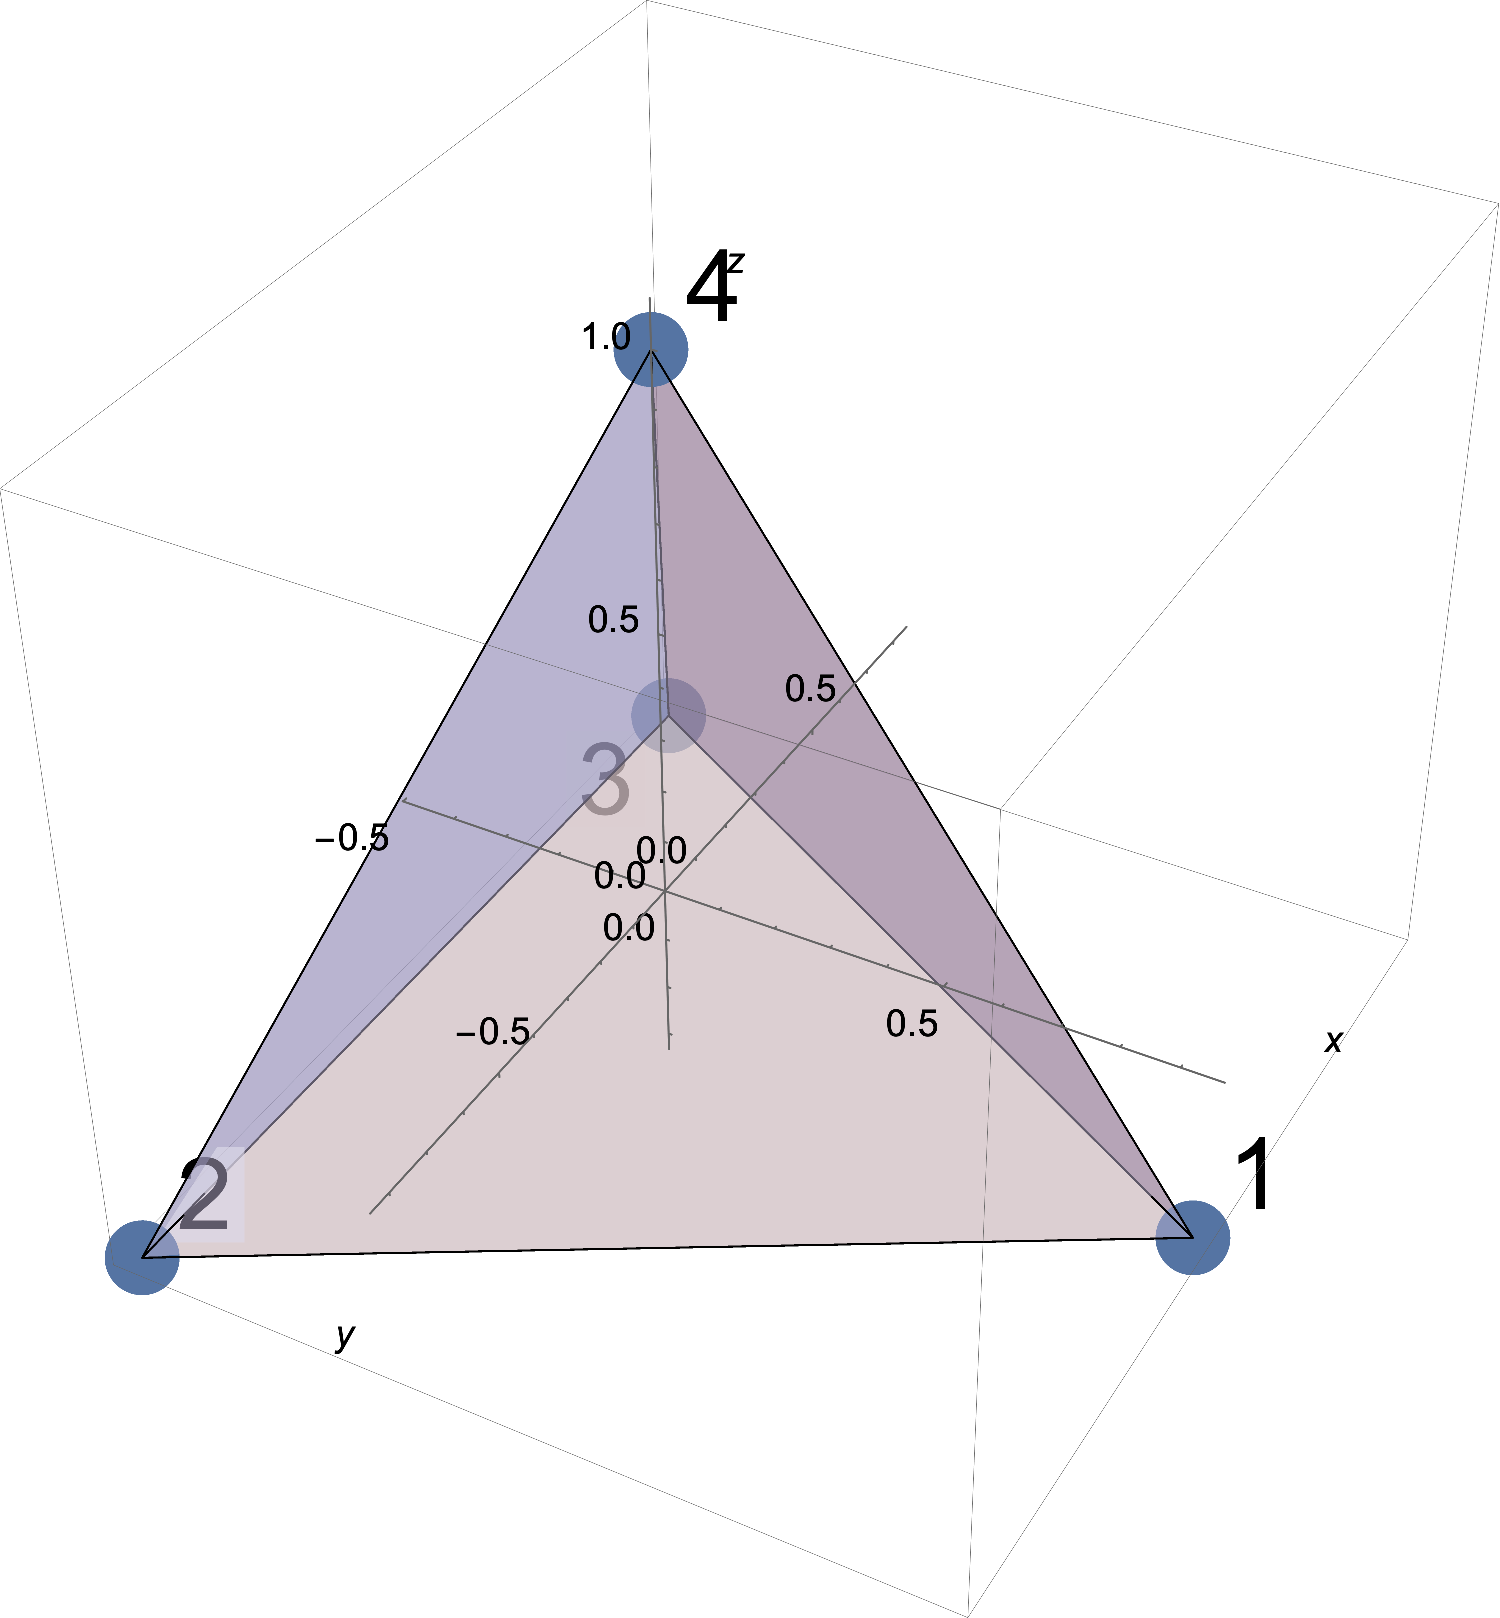
\includegraphics[scale = 0.5]{/Users/philipp/Documents/Studium/Stage/mathematica/id_pos.png}
	\caption{La position du nageur 4S correspondante à l'identité}
	\label{fig:globalintensity_china}
\end{figure}


\section{Symétrie rotationnelle}

\begin{lemma}
A un point $R \in SO(3)$ l'espace tangent est donné par
\begin{align*}
	R^* \asym_3(\R) = \{RA \mid A \in \asym_3(\R)\},
\end{align*}
où $\asym_3(\R)$ désigne les matrices réelles antisymétriques de taille 3.
\end{lemma}

\begin{proof}
On remarque d'abord qu'il suffit de calculer l'espace tangent à l'identité car $SO(3)$ est un groupe de Lie et donc $SO(3)$ agit sur soi-même par difféomorphismes. En effet, si on connaît l'espace tangent à l'identité, l'espace tangent à un point arbitraire $R \in SO(3)$ est donné par le tire-en-arrière $T_{R}SO(3) = R^{*}T_{I}SO(3)$. De plus, $SO(3)$ est la composante connexe de l'identité de $O(3)$ (par continuité de la déterminante). Par conséquent, nous avons $T_{I}SO(3) = T_{I}O(3)$. Or, d'après le théorème du rang constant, $O(3)$ est défini par $O(3) = \Phi^{-1}(I)$, où $\Phi: GL(\R,3) \to M_{3 \times 3}(R)$ est donné par $\Phi(A) = A^T A$. Pour $Q \in GL(\R,3)$, la différentielle $d_{Q} \Phi: T_QO(3) \to T_{Q^TQ}M_{3 \times 3}(\R)$ est donnée par $R \mapsto RQ + QR^T$, en particulier à l'identité nous avons $d_I \Phi(R) = R + R^T$. Il suit d'un corollaire du théorème du rang constant que
\begin{align*}
	T_I O(3) = \ker d_I \Phi = \{R \in M_{3 \times 3}(\R) \mid R + R^T = 0\} = \asym_3(\R).
\end{align*}
\end{proof}

Avec ce lemme, on trouve que pour tout $p = (\mathbf{c} ,R) \in \mathcal{P}$ on a $T_p \mathcal{P} \simeq \R^3 \times R^{*}\asym_3(\R)$. En particulier, on peut écrire le système (\ref{eq:control_problem}) sous la forme 
\begin{align*}
\dot{p} = F(R, \xi) \dot{\xi} = (F_c(R, \xi) \dot{\xi}, F_\theta(R, \xi) \dot{\xi}),
\end{align*}
où  $F_c(R, \xi) \in M_{3 \times 4}(\R)$ et $F_\theta(R, \xi) \in \mathcal{L}(\R^4, R^* \asym_3(\R))$.

Soit maintenant $p_0 = (c_0, R_0)$ une position initiale et $\xi: I \subset \R \to \M$ une courbe de contrôle avec $I$ un voisinage de zéro et $\xi_0 := \xi(0)$. Soit $\gamma(p_0, \xi) = (\gamma_c(p_0, \xi), \gamma_\theta(p_0, \xi))$ la solution associée au système (\ref{eq:control_problem}) avec condition initiale $p(0) = p_0$. Il suit de l'invariance rotationnelle des équations de Stokes que pour tout $R\in SO(3)$
\begin{align}
\label{eq:spatial_rot_inv}
	\gamma_c(c_0, R R_0, \xi)(t) &= R \gamma_c(c_0, R_0, \xi)(t) + (I - R)c_0\\
\label{eq:ang_rot_inv}
	\gamma_\theta(c_0, R R_0, \xi)(t) &= R \gamma_{\theta}(c_0,R_0, \xi)(t)
\end{align}


\begin{proposition}
\label{prop:rot_inv}
Soit $\xi_0 := \xi(0) \in \M$ l'état initial des paramètres de contrôle et $T_{\xi} \M$ l'espace tangent de $\M$ à $\xi$. Si le système de contrôle (\ref{eq:control_problem}) est invariant sous rotations et si $T_{\xi} \M \simeq \R^4$, alors
\begin{align*}
	F(R, \xi) =  (R F_{c}(\xi), R F_{\theta}(\xi) )& & \text{ avec } & & F_{c}(\xi):= F_{c}(I, \xi), F_{\theta}(\xi) := F_{\theta}(I, \xi)
\end{align*}
pour tout $(R, \xi) \in SO(3) \times \M$.
\end{proposition}

\begin{proof}
Par définition du système (\ref{eq:control_problem}) on a
\begin{align*}
	\dot{\gamma}_{c}(c_0, R R_0, \xi)(t) &= F_{c} \left ( \gamma_{\theta}(c_0, R R_0, \xi), \xi \right ) \dot{\xi}(t),\\
	\dot{\gamma}_{\theta}(c_0, R R_0, \xi)(t) &= F_{\theta} \left ( \gamma_{\theta}(c_0, R R_0, \xi), \xi\right ) \dot{\xi}(t)
\end{align*}
Par (\ref{eq:spatial_rot_inv}) et (\ref{eq:ang_rot_inv}), on a également par définition du système
\begin{align*}
	\dot{\gamma}_{c}(c_0, R R_0, \xi)(t) &= R F_{c}(\gamma_{\theta}(c_0,R_0,  \xi), \xi) \dot{\xi}(t)\\
	\dot{\gamma}_{\theta}(c_0, R R_0, \xi)(t) &= R F_{\theta}(\gamma_{\theta}(c_0, R_0, \xi), \xi) \dot{\xi}(t)
\end{align*}
\
Ainsi, on trouve pour tout $R \in SO(3)$
\begin{align*}
	F_{c} \left ( \gamma_{\theta}(c_0, R R_0, \xi),  \xi \right ) \dot{\xi} &= R F_{c}(\gamma_{\theta}(c_0, R_0, \xi), \xi) \dot{\xi}\\
	F_{\theta} \left ( \gamma_{\theta}(c_0, R R_0, \xi), \xi\right ) \dot{\xi} &= R F_{\theta}(\gamma_{\theta}(c_0, R_0, \xi), \xi) \dot{\xi},
\end{align*}
Vu que $T_{\xi}\M \simeq \R^4$, évaluation à $t = 0$ de cette dernière expression fournit $F_{c}(R \, R_0, \xi_0) = RF_{c}(R_0, \xi_0)$ et $F_{\theta}(R \, R_0, \xi_0) = R F_{\theta}(R_{0}, \xi_0)$. Finalement, si on définit $R_0 = I$, on obtient le résultat souhaité.
\end{proof}

\section{Permutation des bras}
D'abord, on définit les matrices de permutations suivantes:
\begin{align*}
	L = (e_2 \mid e_1 \mid e_3 \mid e_4) & & M = (e_1 \mid e_3 \mid e_2 \mid e_4) & &
	N = (e_1 \mid e_2 \mid e_4 \mid e_3)
\end{align*}
où si on les applique à $\M$, les matrices $L, M, N$ et $O$ correspondent aux permutations des bras $||1\leftrightsquigarrow ||2, ||2\leftrightsquigarrow ||3, ||$ et 
$3\leftrightsquigarrow ||4$ respectivement. On notera $S_{xy}(\phi)$ la réflexion à un plan orthogonal au plan $xy$ faisant un angle $\phi$ avec l'axe $x$. On notera $S_{yz}(\phi)$ l'analogue pour le plan $yz$. De plus, on remarque pour la suite que l'angle entre deux bras d'un tétraèdre, \emph{l'angle du tétraèdre}, est donné par
\begin{align*}
	\alpha_{tet} = \arccos(-1/3).
\end{align*}
Comme pour l'invariance rotationnelle on traitera la partie spatiale et la partie angulaire séparément.

\subsection{Symétrie spatiale}
Pour chaque permutation on fixe une orientation de référence $R_L, R_M$ et $R_N$ respectivement de sorte que les deux bras en question soient symétrique par rapport au plan $yz$. Pour alléger la notation, on écrit $S := S_{xy}(\tfrac{\pi}{2})$. De plus, on pose  $R_{L} = R_{z}(-\pi/6), R_{M} = R_{z}(\pi/2)$ et $R_{N} = R_{z}(-\pi/6)R_{y}(-\alpha_{tet})$. Finalement, on fixe pour toutes les trois permutations une position spatiale de référence $c_{\mathrm{ref}} \in \R^3$. Soient alors $\gamma(c_{\mathrm{ref}}, R_L, L\xi), \gamma(c_{\mathrm{ref}}, R_M, M\xi)$ et $\gamma(c_{\mathrm{ref}}, R_N, N\xi)$ des solutions du système de contrôle.
Ainsixx, on trouve grâce à l'invariance sous changement de point d'observations des équations de Stokes, i.e. en regardant les solutions dans un miroir, les relations
\begin{equation}
\label{eq:spat_perm_inv}
\begin{aligned}
		\gamma_c(c_{\mathrm{ref}}, R_L, L \xi) &= S\gamma_{c}(S c_{\mathrm{ref}}, R_L, \xi)\\
		\gamma_c(c_{\mathrm{ref}}, R_M, M \xi) &= S\gamma_{c}(Sc_{\mathrm{ref}}, R_M, \xi) \\
		\gamma_c(c_{\mathrm{ref}}, R_N, N \xi) &= S \gamma_{c}(Sc_{\mathrm{ref}}, R_N, \xi).
\end{aligned}
\end{equation}




Soit $p_0 = (c_o, R_0) \in \mathcal{P}$ une position initiale et $\gamma_{c}(c_0, R_0, L \xi)$ la partie spatiale de la solution du problème de contrôle. Pour tout $R \in SO(3)$, on a par (\ref{eq:spatial_rot_inv})
\begin{align*}
	\gamma_{c}(c_0, R_0, L \xi) = R^{-1} \gamma_{c}(c_0, R R_0, L \xi) - (R^{-1} - I) c_0.
\end{align*}
Soit $R_1 := R_{L}R_0^{-1}$. Par la condition (\ref{eq:spat_perm_inv}), on a
\begin{align*}
	\gamma_{c}(c_0, R_0, L \xi)(t) = R_{1}^{-1} S \gamma_c (Sc_0, R_{L}, \xi)(t) - (R^{-1}_1 - I) c_0.
\end{align*}
Ainsi, on trouve par définition du système et avec la proposition \ref{prop:rot_inv}
\begin{align*}
	\dot{\gamma}_c (c_0, R_0, \xi)(t)
	 &= \gamma_{\theta}(c_0, R_0, \xi)(t) F_c(L \xi) L \dot{\xi}(t)\\
	 &= R_{1}^{-1} S \gamma_{\theta}(Sc_0, R_{L}, \xi)(t) F_{c}(\xi) \dot{\xi}(t).
\end{align*}
Évaluation à $t = 0$ et le fait que $T_{\xi}\M \simeq \R^4$ pour tout $\xi \in \M$ fournissent 
\begin{align*}
	R_0 F_c(L \xi_0) L = R_{1}^{-1} S R_{L} F_c(\xi_0).
\end{align*}
En posant $S_L := R_{L}^{-1} S R_{L}$, on trouve alors $F_c(L \xi) = S_L F_c(\xi) L$ pour tout $\xi \in \M$. En particulier, ce calcul fonctionne de même pour les autres permutations et en posant
\begin{align*}
	S_{M} := R_{M}^{-1} S R_{M} & & S_{N} := R_{N}^{-1} S R_{N}
\end{align*}
nous avons alors démontré le résultat suivant.

\begin{proposition}
\label{prop:spat_perm_inv}
Pour toute courbe de contrôle $\xi$, l'application $F_c$ satisfait
\begin{align*}
	F_c(L \xi) = S_L F_c(\xi) L & &F_c(M \xi) = S_M F_c(\xi) M & &F_c(N \xi) = S_N F_c(\xi) N.
\end{align*}
\end{proposition}

\subsection{Symétrie angulaire}
On commence par quelques observations concernant la réflexion d'une rotation à un plan. Jusque là, nous avons identifié $SO(3)$ aux matrices orthogonales de déterminante 1. Or, le théorème d'Euler dit que pour toute rotation dans $SO(3)$ il existe une axe de rotation $\mathbf{u} \in S^2$ de sorte que l'on puisse la représenter par le vecteur d'Euler $\mathbf{\omega} = \theta \mathbf{u}$, où $\theta$ est l'angle de rotation. Le lien entre ces deux représentations est donné par l'exponentielle matricielle que l'on explicitera dans ce qui suit. On se rappelle que
\begin{align*}
	\so(3) = T_{I}SO(3) = \asym_3(\R).
\end{align*}
De plus, on notera $R_{x}(\theta), R_{y}(\theta)$ et $R_{z}(\theta)$ les rotations élémentaires autour des axes $x,y$ et $z$, respectivement. On voit facilement que $\dim \asym_3(\R) = 3$ et on trouve que les matrices
\begin{align*}
	&L_1 = \frac{d}{d\theta}R_x(\theta)_{\mid \theta =0} = \left(\begin{array}{ccc}
	0 & 0 & 0 \\ 
	0 & 0 & -1 \\ 
	0 & 1 & 0
	\end{array}  \right ),\\
	&L_2 = \frac{d}{d\theta}R_y(\theta)_{\mid \theta =0} = \left (\begin{array}{ccc}
	0 & 0 & 1 \\ 
	0 & 0 & 0 \\ 
	-1 & 0 & 0
	\end{array}  \right ),\\
	&L_3 = \frac{d}{d\theta}R_z(\theta)_{\mid \theta =0} = \left (\begin{array}{ccc}
	0 & -1 & 0 \\ 
	1 & 0 & 0 \\ 
	0 & 0 & 0
	\end{array}  \right ),
\end{align*}
forment une base de $\so(3)$ que l'on notera $\mathcal{L}$. Pour $A \in \so(3)$ on obtient avec les propriétés de l'exponentielle matricielle que
\begin{align*}
	(e^{A})^T e^{A} = e^{A^T} e^{A} = e^{-A} e^{A} = e^{I} = I.
\end{align*}
Donc, cette application est bien-définie et en particulier on a $R_z(\theta) = e^{\theta L_z}$ et similaire pour les autres rotations similaires. On remarque que pour tout $A \in \so(3)$ et $Q \in SO(3)$ on a $QAQ^T \in \so(3)$. Soit maintenant $R \in SO(3)$ quelconque. On trouve toujours un $Q \in SO(3)$ de sorte que
\begin{align*}
	R = Q R_{z}(\theta) Q^T = Q e^{\theta L_z} Q^{T} = e^{\theta QL_zQ^{T}} = e^{\theta \mathbf{u} \cdot \mathbf{L}},
\end{align*}
avec $\mathbf{L} = (L_x, L_y, L_z)^T$ où on permet un petit abus de notation et $\mathbf{u} \in S^2$ car $Q$ est une application orthogonale. Ceci montre bien que $\exp: \so(3) \to SO(3)$ est surjectif. Réciproquement, le calcul direct montre que pour une axe de rotation $\mathbf{u} \in S^2$ et un angle de rotation $\theta \in \R$ la matrice $R = \exp(\theta \mathbf{u} \cdot \mathbf{L})$ est bien la matrice de rotation associée.


Soit $S$ une réflexion à un plan dans $\R^3$ et $R \in SO(3)$ l'orientation d'un corps rigide dans $\R^3$ avec vecteur d'Euler $\omega$ associé. On notera $\tilde{R} \in SO(3)$ l'orientation de l'image miroir du corps rigide avec vecteur d'Euler $\tilde{\omega}$. On s'aperçoit que $\tilde{\omega} = -S \omega$, i.e. l'axe de rotation est reflétée et au même temps le sens de rotation est inversé pour les rotations parallèles au plan de réflexion. Un petit calcul montre que
\begin{align}
\label{eq:rep_ref}
\tilde{\omega} \cdot \mathbf{L} = S(\omega \cdot \mathbf{L})S,
\end{align}
dont il suit que
\begin{align}
	\tilde{R} = \exp(\tilde{\omega} \cdot \mathbf{L}) = \exp(S(\omega \cdot \mathbf{L}) S) = S R S.
\end{align}

Maintenant, on se donne une orientation de référence $R_{\mathrm{ref}} := R_z(-\tfrac{\pi}{6})$ ainsi que les réflexions $T_L := S_{xy}(\tfrac{\pi}{2}), T_{M} := S_{xy}(\tfrac{5\pi}{6})$ et $T_{N} := S_{yz}((\pi - \alpha_{tet})/2)$. De nouveau par l'invariance sous changement de point de vue des équations de Stokes justifient les relations suivantes, où on a directement compensé pour la position initiale.
\begin{equation}
\label{eq:ang_perm_inv}
\begin{aligned}
	\gamma_{\theta}(c_{\mathrm{ref}}, R_{\mathrm{ref}}, L \xi) &= R_{\mathrm{ref}} T_{L} R_{\mathrm{ref}}^{-1} \gamma_{\theta}(T_{L} c_{\mathrm{ref}}, R_{\mathrm{ref}}, \xi) T_{L}\\
	\gamma_{\theta}(c_{\mathrm{ref}}, R_{\mathrm{ref}}, M \xi) &= R_{\mathrm{ref}} T_{M} R_{\mathrm{ref}}^{-1} \gamma_{\theta}(T_{M}c_{\mathrm{ref}}, R_{\mathrm{ref}}, \xi) T_{M}\\
	\gamma_{\theta}(c_{\mathrm{ref}}, R_{\mathrm{ref}}, N \xi) &= R_{\mathrm{ref}} T_{N} R_{\mathrm{ref}}^{-1} \gamma_{\theta}(T_{N}c_{\mathrm{ref}}, R_{\mathrm{ref}}, \xi) T_{N}.
\end{aligned}
\end{equation}
Soit $p_0  = (c_0, R_0) \in \mathcal{P}$ une position initiale. Alors, nous avons par (\ref{eq:ang_rot_inv}) pour tout $R \in SO(3)$
\begin{align*}
	\gamma_{\theta}(c_0, R_0, L \xi) = R^{-1}\gamma_{\theta}(c_0, R R_0, L\xi).
\end{align*}
En particulier, pour $R_1 := R_{\mathrm{ref}} R_{0}^{-1}$ on obtient avec la condition (\ref{eq:ang_perm_inv})
\begin{equation}
\begin{aligned}
	\gamma_{\theta}(c_0, R_0, L \xi) &= R_{1}^{-1} \gamma_{\theta}(c_0, R_{\mathrm{ref}}, L \xi)\\
	 &= R_{1}^{-1} R_\mathrm{ref} T_{L} R_{\mathrm{ref}}^{-1}\gamma_{\theta}(T_{L}c_0, R_{\mathrm{ref}}, \xi) T_{L}.
\end{aligned}
\end{equation}
Par définition du système et en utilisant la proposition \ref{prop:rot_inv}, on obtient à $t = 0$
\begin{align}
	F_{\theta}(L \xi_0) L \dot{\xi}(0) = T_{L} F_{\theta}(\xi_0) \dot{\xi}(0) T_{L}.
\end{align}

On continue par représenter $F_{\theta}(\xi_0) \in \mathcal{L}(\R^4, \asym_3(\R))$ par une matrice $[F_{\theta}(\xi_0)]_{\mathcal{E}}^{\mathcal{L}} \in M_{3 \times 4}(\R)$ par rapport aux bases $\mathcal{L}$ et $\mathcal{E} = (e_1, e_2, e_3,e_4)$. En particulier, le calcul de (\ref{eq:rep_ref}) montre que la la matrice représentant l'application linéaire $A \in \asym_3(\R) \mapsto T_{L} A T_{L} \in \asym_3(\R)$ est donnée par $-T_{L}$ dans la base $\mathcal{L}$. Donc, nous avons par rapport aux bases $\mathcal{E}$ et $\mathcal{L}$
\begin{align*}
	&[F_{\theta}(L \xi_0) L \dot{\xi}(0)]_{\mathcal{E}}^{\mathcal{L}} = [F_{\theta}(L \xi_0)]_{\mathcal{E}}^{\mathcal{L}} L [\dot{\xi}(0)]_{\mathcal{E}},\\
	&[T_L F_{\theta}(\xi_0)\dot{\xi}(0)T_L]_{\mathcal{L}} = -T_L[F_{\theta}(\xi_0) \dot{\xi}(0)]_{\mathcal{L}} = - T_L [F_{\theta}(\xi_0)]_{\mathcal{E}}^{\mathcal{L}} [\dot{\xi}(0)]_{\mathcal{E}},
\end{align*}
et donc $[F_{\theta}(L \xi)]_{\mathcal{E}}^{\mathcal{L}} = - T_L [F_{\theta}(\xi)]_{\mathcal{E}}^{\mathcal{L}} L$ car $T_{\xi} \M \simeq \R^4$ pour tout $\xi \in \M$. Le calcul pour les autres permutations se déroule de la même façon et donc nous avons démontré le résultat suivant.
\begin{proposition}
\label{prop:ang_perm_inv}
Pour toute courbe de contrôle $\xi$, l'application $F_{\theta}$ satisfait
\begin{align*}
	[F_{\theta}(L \xi)]_{\mathcal{E}}^{\mathcal{L}} &= - T_{L} [F_{\theta}(\xi)]_{\mathcal{E}}^{\mathcal{L}} L, & [F_{\theta}(M \xi)]_{\mathcal{E}}^{\mathcal{L}} = - T_{M} [F_{\theta}(\xi)]_{\mathcal{E}}^{\mathcal{L}} M,\\	
	[F_{\theta}(N \xi)]_{\mathcal{E}}^{\mathcal{L}} &= - T_{N} [F_{\theta}(\xi)]_{\mathcal{E}}^{\mathcal{L}} N.
\end{align*}
\end{proposition}

\section{Développement limité du système de contrôle}



Soit $G: \M \to M_{3 \times 4}(\R)$ une application analytique. On pose $\zeta = \xi_0 + \xi$, où $\xi_0 \in \M$ avec toutes composantes égales. De plus, on pose $G_{\xi_0}(\xi) := G(\xi_0 + \xi)$. Ainsi, nous pouvons écrire le développement limité pour $\eta \in \R^4$
\begin{align}
\label{eq: general_expansion}
	G_{\xi_0}(\xi)\eta = G_0 \eta + \h_{0}(\xi \otimes \eta) + \mathcal{O}(|\xi|^2) \eta,
\end{align}
où $G_0 := G(\xi_0) \in M_{3 \times 4}(\R)$ et $\h_{0}\in \mathcal{L}(\R^4 \otimes \R^4, \R^3)$ représente la différentielle d'ordre un de $G_{\xi_0}$ à $\xi = 0$. Le résultat suivant sera utile dans la suite:

\begin{proposition}
\label{prop:general_expansion}
Soient $A \in M_{4 \times 4}(\R)$ et $S_A \in M_{3 \times 3}(\R)$ des matrices telles que $G(A \xi) = S_A G(\xi) A$ pour tout $\xi \in \R^4$. Alors, on a
\begin{align}
\label{eq: general_zeroth_term}
	G_0 = S_A G_0 A
\end{align}
ainsi que 
\begin{align}
\label{eq: general_firstord_term}
	\h_0((A \xi) \otimes \eta) = S_A \h_{0}(\xi \otimes (A \eta))
\end{align}
pour tout $\xi, \eta \in \R^4$.
\end{proposition}

\begin{proof}
Évaluation de la relation $G(A \xi) = S_A G(\xi) A$ à $\xi = 0$ fournit immédi-\linebreak atement (\ref{eq: general_zeroth_term}). Puis, on pose $\eta := A \eta$ dans (\ref{eq: general_expansion}) et on obtient
\begin{align}
\label{eq: general_expansion_proof1}
	G_{\xi_0}(\xi)A\eta = G_0 A \eta + \h_0(\xi \otimes A\eta) + \mathcal{O}(|\xi|^2)\eta.
\end{align}
Par conséquent, on déduit de (\ref{eq: general_expansion}) et (\ref{eq: general_expansion_proof1}) que
\begin{align*}
	\h_0((A \xi) \otimes \eta) &\overset{(\ref{eq: general_expansion})}{=} G_{\xi_0}(A \xi)\eta - G_0 \eta + \mathcal{O}(|\xi|^2) \eta\\
	&= S_A G_{\xi_0}(\xi)A \eta - G_0 \eta + \mathcal{O}(|\xi|^2)\eta\\
	&= S_A[G_{0}A \eta + \h_0(\xi \otimes (A \eta))] - G_0 \eta + \mathcal{O}(|\xi|^2)\eta\\
	&= S_A \h_0(\xi \otimes (A \eta)) + \mathcal{O}(|\xi|^2)\eta,
\end{align*}
et donc on a (\ref{eq: general_firstord_term}).
\end{proof}

Dans la suite, on identifiera la matrice $[F_{\theta}(\xi)]_{\mathcal{E}}^{\mathcal{L}} \in M_{3 \times 4}(\R)$ à l'application $F_{\theta}(\xi) \in \mathcal{L}(\R^4, \asym_3(\R))$ car aucune confusion ne peut plus survenir. Ainsi, nous avons les deux fonctions $F_{c}, F_{\theta}: \M \to M_{3 \times 4}(\R)$ qui sont analytiques. %ref
.
Maintenant on peut écrire les développements limité 
\begin{align}
	F_{c,\xi_0}(\xi)\eta &= F_{c,0} \eta + \h_{c,0}(\xi \otimes \eta) + \mathcal{O}(|\xi|^2) \eta,\\
	F_{\theta,\xi_0}(\xi)\eta &= F_{\theta,0} \eta + \h_{\theta,0}(\xi \otimes \eta) + \mathcal{O}(|\xi|^2) \eta
\end{align}
 En particulier, les propositions (\ref{prop:spat_perm_inv}), (\ref{prop:ang_perm_inv}) et (\ref{prop:general_expansion}) fournissent les relations suivantes pour les termes d'ordre zéro
\begin{align}
\label{eq:spat_perm_inv_ord0}
	S_L F_{c,0} L &= F_{c,0} &  S_{M} F_{c,0} M &= F_{c,0} &  S_{N} F_{c,0} N &= F_{c,0}\\
\label{eq:ang_perm_inv_ord0}
	- T_L F_{\theta,0} L &= F_{\theta,0}, &  -T_M F_{\theta,0}M &= F_{\theta,0} , &  -T_N F_{\theta,0}N &= F_{\theta,0} .
\end{align}
et pour les termes d'ordre 1
\begin{equation}
\label{eq:spat_sym_first_order}
	\begin{aligned}
	\h_{c,0}((L \xi) \otimes \eta) &= S_{L}\h_{c,0}(\xi \otimes (L \eta)), & \h_{\theta,0}((L\xi) \otimes \eta) &=  -T_L \h_{\theta,0}(\xi \otimes (L \eta))\\
	 \h_{c,0}((M \xi) \otimes \eta) &= S_{M}\h_{c,0}(\xi \otimes (M \eta)), & \h_{\theta,0}((M\xi) \otimes \eta) &=  -T_M \h_{\theta,0}(\xi \otimes (M \eta))\\	 
	\h_{c,0}((N \xi) \otimes \eta) &= S_{N}\h_{c,0}(\xi \otimes (N \eta)), & 	\h_{\theta,0}((N\xi) \otimes \eta) &=  -T_N \h_{\theta,0}(\xi \otimes (N \eta)).
	\end{aligned}
\end{equation}


\section{Résolution des systèmes}
\subsection{Les termes d'ordre zéro}
Pour la partie spatiale on applique juste les relations (\ref{eq:spat_perm_inv_ord0}) à une matrice générique dans $M_{3 \times 4}(\R)$ pour trouver
\begin{equation}
	F_{c,0} = \left ( \begin{array}{cccc}
	- 2 \mathfrak{a}  & \mathfrak{a}  & \mathfrak{a}  & 0 \\ 
	0 & \sqrt{3}\mathfrak{a}  & -\sqrt{3}\mathfrak{a}  & 0 \\ 
	 \tfrac{1}{\sqrt{2}}\mathfrak{a} & \tfrac{1}{\sqrt{2}}\mathfrak{a} & \tfrac{1}{\sqrt{2}} \mathfrak{a}  & \tfrac{-3}{\sqrt{2}}\mathfrak{a} 
	\end{array} \right ),
\end{equation}
pour un $\mathfrak{a} \in \R$. On remarque que la partie de la matrice correspondante aux bras 1,2 et 3 et aux directions $x$ et $y$ est égale au terme d'ordre zéro pour le nageur 3S. De plus, les vecteurs $\tau_1 : = \tfrac{1}{\sqrt{6}}(-2,1,1,0)^T$, $\tau_2 := \tfrac{1}{\sqrt{2}}(0,1,-1,0)^T$, $\tau_{3}:= \tfrac{1}{2 \sqrt{3}} (1,1,1,-3)^T$ et $\tau_4:= \tfrac{1}{2}(1,1,1,1)^T$ forment une base orthonormée en termes de laquelle $F_{c,0}$ s'écrit $F_{c,0} = \mathfrak{a} \sqrt{6} [\tau_1 | \tau_2 | \tau_3]^T$.

Pour la partie angulaire, le même calcul direct montre que $F_{\theta,0} = 0$ ce qui se voit déjà avec l'argument géométrique que dans une configuration symétrique des bras, il n'y aura pas de couple.



\subsection{Les termes de premier ordre}
On notera $\sigma_{L} = (2,1), \sigma_{M} = (2,3)$ et $ \sigma_{N} = (3,4)$ de $S_4$ les permutations correspondantes à $L, M$ et $N$, respectivement, i.e. pour la base ordonnée $(e_1, e_2, e_3, e_4)$ on a $Le_i = e_{\sigma_L(i)}$ etc. Ainsi, en évaluant sur la base ordonnée,  (\ref{eq:spat_sym_first_order}) s'écrit
\begin{align}
\label{eq:basis_rel_spat_first_ordL}
	\h_{c,0}(e_{\sigma_L(i)} \otimes e_{j}) &= S_{L}\h_{c,0}(e_i \otimes e_{\sigma_L(j)})\\
\label{eq:basis_rel_spat_first_ordM}
	\h_{c,0}(e_{\sigma_{M}(i)} \otimes e_j) &= S_{M}\h_{c,0}(e_{i} \otimes e_{\sigma_{M}(j)})\\
\label{eq:basis_rel_spat_first_ordN}
	\h_{c,0}(e_{\sigma_{N}(i)}\otimes e_{j}) &= S_{N}\h_{c,0}(e_{i}\otimes e_{\sigma_{N}(j)}),
\end{align}
pour tout $i,j \in \N_4$. Ceci fournit un système de $48$ équations vectorielles. En effet, chaque $\h_{c,0}(e_i \otimes e_j)$ est un vecteur dans $\R^3$. Or, on remarque que les matrices $S_{L}, S_{M}$ et $S_{L}$ sont idempotentes, c'est-à-dire que l'on a également les équations $S_{L} \h_{c,0}(e_{\sigma_L(i)} \otimes e_{j}) = \h_{c,0}(e_i \otimes e_{\sigma_L(j)})$ pour tout $i,j \in \N_{4}$ et similaire pour $M$ et $N$. Ceci réduit le système à $30$ équations vectorielles. On pose $A_k = (\h_{c,0}(e_i \otimes e_j) \cdot e_k)_{i,j \in \N_4}$ pour $k \in \N_{3}$. Ainsi, le vecteur $\h_{c,0}(\xi \otimes \eta) \in \R^3$ s'écrit pour tout $\xi, \eta \in \R^4$
\begin{align*}
	\h_{c,0}(\xi \otimes \eta) = \sum_{k \in \N_3} (A_k\eta \cdot \xi)e_k.
\end{align*}
En posant
\begin{align*}
	\alpha = \frac{1}{2} \h_{c,0}(e_1 \otimes e_4)\cdot e_1 - \frac{\sqrt{2}}{2} \h_{c,0}(e_1 \otimes e_4)\cdot e_3,
\end{align*}
ainsi que $\beta = -\frac{1}{4} \h_{c,0}(e_1 \otimes e_4)\cdot e_1 + \frac{\sqrt{2}}{2} \h_{c,0}(e_1 \otimes e_4)\cdot e_3$, $\gamma = \frac{\sqrt{2}}{2} \h_{c,0}(e_1 \otimes e_2)\cdot e_3$ et $\lambda = -\frac{3}{2} \h_{c,0}(e_1 \otimes e_1)\cdot e_1$ on obtient à l'aide des relations (\ref{eq:basis_rel_spat_first_ordL}) - (\ref{eq:basis_rel_spat_first_ordN})

\renewcommand{\arraystretch}{1.3}
\begin{align}
	A_1 &= \frac{1}{3} \left(
\begin{array}{cccc}
 -2 \lambda & 2 (\alpha+2 (\beta+\gamma)) & 2 (\alpha+2 (\beta+\gamma)) & 6 (\alpha+\gamma) \\
 2 (\alpha-\beta+2 \gamma) & \lambda& -4 \alpha-6 \gamma & -3 (\alpha+\gamma) \\
 2 (\alpha-\beta+2 \gamma) & -4 \alpha-6 \gamma & \lambda & -3 (\alpha+\gamma) \\
 4 (\alpha+2 \gamma) & -\alpha-3 \gamma & -\alpha-3 \gamma & 0 \\
\end{array}
\right), \\
	A_2 &= \frac{1}{\sqrt{3}} \left(
\begin{array}{cccc}
 0 & -2 (\alpha+2 \gamma) & 2 (\alpha+2 \gamma) & 0 \\
 -2 (\alpha+\beta+2 \gamma) & \lambda & -2 \alpha & -3 (\alpha+\gamma) \\
 2 (\alpha+\beta+2 \gamma) & 2 \alpha & -\lambda & 3 (\alpha+\gamma) \\
 0 & -\alpha-3 \gamma & \alpha+3 \gamma & 0 \\
\end{array}
\right) ,\\
	A_3 &= \frac{1}{3 \sqrt{2}} \left(
\begin{array}{cccc}
 \lambda & -2 (2 \alpha+\beta+4 \gamma) & -2 (2 \alpha+\beta+4 \gamma) & 6 \gamma \\
 -2 (2 \alpha+\beta+4 \gamma) & \lambda& -4 \alpha-6 \gamma & 6 \gamma \\
 -2 (2 \alpha+\beta+4 \gamma) & -4 \alpha-6 \gamma& \lambda & 6 \gamma \\
 4 \alpha+6 \beta+8 \gamma & 8 \alpha+6 \gamma & 8 \alpha+6 \gamma & -3 \lambda \\
\end{array}
\right)
\end{align}
\renewcommand{\arraystretch}{1.0}
Ainsi, on trouve pour les parties anti-symétriques $M_k := \tfrac{1}{2}(A_k - A_k^T), k \in \N_3$
\renewcommand{\arraystretch}{1.3}
\begin{align}
	M_1 &= \frac{1}{3} \left(
\begin{array}{cccc}
 0 & 3 \beta & 3 \beta & \alpha-\gamma\\
 -3 \beta & 0 & 0 & -\alpha \\
 -3 \beta & 0 & 0 & -\alpha \\
 \gamma-\alpha & \alpha & \alpha & 0 \\
\end{array}
\right) ,\\
	M_2 &= \frac{1}{\sqrt{3}} \left(
\begin{array}{cccc}
 0 & \beta & -\beta & 0 \\
 -\beta & 0 & -2 \alpha & -\alpha \\
 \beta & 2 \alpha & 0 & \alpha \\
 0 & \alpha & -\alpha & 0 \\
\end{array}
\right),\\
	M_3 &= \frac{1}{3 \sqrt{2}} \left(
\begin{array}{cccc}
 0 & 0 & 0 & -2 \alpha-3 \beta-\gamma \\
 0 & 0 & 0 & -4 \alpha \\
 0 & 0 & 0 & -4 \alpha\\
 2 \alpha+3 \beta+\gamma & 4 \alpha & 4 \alpha & 0 \\
\end{array}
\right)
\end{align}
\renewcommand{\arraystretch}{1.0}
Avec la même notation, on trouve pour la partie angulaire le système
\begin{align}
\label{eq:basis_rel_ang_first_ordL}
	\h_{\theta,0}(e_{\sigma_L(i)} \otimes e_{j}) &= -T_{L}\h_{\theta,0}(e_i \otimes e_{\sigma_L(j)})\\
\label{eq:basis_rel_ang_first_ordM}
	\h_{\theta,0}(e_{\sigma_{M}(i)} \otimes e_j) &= -T_{M}\h_{\theta,0}(e_{i} \otimes e_{\sigma_{M}(j)})\\
\label{eq:basis_rel_ang_first_ordN}
	\h_{\theta,0}(e_{\sigma_{N}(i)}\otimes e_{j}) &= -T_{N}\h_{\theta,0}(e_{i}\otimes e_{\sigma_{N}(j)}),
\end{align}
ce qui se réduit aussi à un système de 30 équations vectorielles car les matrices $T_L, T_{M}$ et $T_N$ sont bien idempotentes. On pose $B_k = (\h_{\theta,0}(e_i \otimes e_j) \cdot e_k)_{i,j \in \N_4}$ pour $k \in \N_{3}$. En posant $\delta := \mathcal{H}_{\theta, 0}(e_1 \otimes e_4) \cdot e_1$, on trouve à l'aide des relations (\ref{eq:basis_rel_ang_first_ordL}) - (\ref{eq:basis_rel_ang_first_ordN}) et un calcul très similaire à celui de la partie spatiale
\renewcommand{\arraystretch}{1.3}
\begin{align}
	B_1 &= \left(
\begin{array}{cccc}
 0 & 0 & -\delta & \delta \\
 0 & 0 & -\delta & \delta \\
 \delta & \delta & 0 & -2 \delta \\
 -\delta & -\delta & 2 \delta & 0 \\
\end{array}
\right)\\
	B_2 &= \frac{1}{\sqrt{3}} \left(
\begin{array}{cccc}
 0 & -2 \delta & -\delta & 3 \delta \\
 2 \delta & 0 & \delta & -3 \delta \\
 \delta & -\delta & 0 & 0 \\
 -3 \delta & 3 \delta & 0 & 0 \\
\end{array}
\right) \\
B_3 &= 2 \sqrt{\frac{2}{3}}\left(
\begin{array}{cccc}
 0 & \delta & -\delta & 0 \\
 -\delta & 0 & \delta & 0 \\
 \delta & -\delta & 0 & 0 \\
 0 & 0 & 0 & 0 \\
\end{array}
\right)
\end{align}
\renewcommand{\arraystretch}{1.0}

\section{Système de contrôle linéarisé}
En résumé, on a démontré dans les sections précédentes que à termes d'ordre élevé près, la dynamique de (4S) est donnée par
\begin{equation}
\label{eq: lin_control_eq}
\begin{aligned}
\begin{cases}
	\dot{c} = RF_{c,0} \dot{\xi} + R \sum_{k \in \N_3} (A_k \dot{\xi} \cdot \xi) e_k\\
	\dot{R} = R \sum_{j \in \N_3}(B_j\dot{\xi} \cdot \xi) L_j.
\end{cases}
\end{aligned}
\end{equation}
En particulier, la partie angulaire est de la forme $\dot{R}(t) = R(t) \Gamma(t)$, i.e. une équation différentielle matricielle avec une matrice non-constante $\Gamma(t)$.

\end{document}

\section{The small strokes regime}
\input{small_strokes}

\section{Energy minimizing strokes}
\input{optimization}

\section{The long arms approximation}
\label{sec:laa}
Despite having characterized the dynamics of \textsc{SPr4} as well as the optimal control curves for any prescribed net displacement, we are still missing the physical parameters $\mathfrak{a}, \alpha, \beta, \delta, \lambda, \kappa$ and $h$. Again inspired by \cite{Alouges2017}, we consider the regime of very long arms compared to the radius $a$ of the spheres $B_i$. To that end, let us review the fluid model. Recall that we neglect the arms such that our fluid domain is given by $\Omega := \bigcup_{i \in \N_4} \overline{B}_i$. The geometry of $\Omega$ is completely determined by the common radius $a$ of the four spheres and the matrix $b = (b_i)_{i \in \N_4}$ having as columns the centers of the spheres.

Since we are considering the swimmer \textsc{SPr4} to be microscopically small, we can assume the Reynolds number to be low such that the governing equations are given by Stokes' equations
\begin{align}
\label{eq:stokes}
\begin{cases}
- \mu \Delta u + \nabla p &= 0 \text{ in } \Omega,\\
\mathrm{div} u  &= 0  \text{ in } \Omega,
\end{cases}
\end{align}
subject to the traction boundary condition $- \boldsymbol\sigma n = f$ on $\partial \Omega$, and to the far-field condition $u(x) = o(|x|^{-1})$ as $|x| \to \infty$. The variables $u$ and $p$ denote the velocity field and the pressure of the fluid, respectively, $\mu$ is the viscosity, $n$ the outer unit normal to $\partial \Omega$ directed towards the interior of the balls, $\boldsymbol \sigma := \mu \nabla^{\mathrm{sym}}u - p I$ the Cauchy stress tensor, and $f$ the traction field on the boundary of the swimmer. The swimmer has a rigid structure. Hence, no-slip boundary conditions are imposed on the spheres, where we recall that the instantaneous velocity on the $i$-th sphere in the state $(\xi, p, \sigma) \in \M \times \mathcal{P} \times \partial B_a $ is given by
\begin{equation}
	u_i(\xi, p, \sigma) = \dot{c} + \omega \times (\xi_i z_i + \sigma) + R z_i \dot{\xi}_i,
\end{equation}
with $\omega$ the axial vector associated to the skew matrix $\dot{R} R^T$. Furthermore, the unique velocity field $u$ solution of (\ref{eq:stokes}) can be expressed, for almost every $x \in \partial \Omega$, by a single-layer potential
\begin{align}
\label{eq:single_layer}
	u(x) = \int_{\partial \Omega} G(x - y) f(y) \dd y, & & G(x) := \frac{1}{8 \pi \mu} \left ( \frac{I}{|x|} + \frac{x \otimes x}{|x|^3} \right ),
\end{align}
where the stokeslet $G$ is the fundamental solution to Stokes' equations.

\subsection{The dynamics of \textsc{SPr4} in the long arms regime}
It is shown in \cite{Alouges2013} that in the limit of very long arms, the interactions of the different spheres simplify considerably, i.e. the integral in (\ref{eq:single_layer}). More specifically, denoting by $f_i$ the total force applied to the $i$-th sphere and again by$b_i$ its center, the velocity on the $i$-th sphere can be expressed at the leading order as
\begin{align}
\label{eq:velocity_field_uniform}
	u_i := u_i(\sigma) = \frac{1}{6 \pi \mu a} f_i + \sum_{j \neq i \N_4} G(b_{ij}) f_j,
\end{align}
where $b_{ij} := b_i - b_j$. In fact, we approximate the part of the velocity on $B_i$ due to the force $f_i$ on $B_i$ by Stokes' law, while one can consider the stokeslet to be constant on the other three spheres. The arms of the swimmer are assumed to have the same initial length $\xi \in \R^+$. So, as stated by (\ref{eq:velocity_field_uniform}), when the $i$-th arm of the swimmer is $\xi_0 + \xi_i$ with $\xi_0 \gg a$, the velocity field $u_i$ associated to the forces $(f_i)_{i \in \N_4}$ is uniform on the boundary of the $i$-th sphere. Thus, without loss of generality, we can interpret the velocity field $u_i$ as applied to the center $b_i$ of the $i$-th ball. Furthermore, due to the negligible inertia, the total viscous force and torque exerted by the surrounding fluid on the swimmer must vanish, i.e. the dynamics must satisfy the balance equations
\begin{eqnarray}
\label{eq:balance_equations}
	\sum_{i \in \N_4} f_i = 0, & & \sum_{i \in \N_4} (b_i - c) \times f_i = 0.
\end{eqnarray}
For any $k \in \N_3$, the map $f \mapsto \omega_k(b_i, f) := ((b_i - c) \times f) \cdot \hat{e}_k$ defines a linear form on $\R^3$, where $(\hat{e}_1, \hat{e}_2, \hat{e}_3)$ denotes the standard basis of $\R^3$. Hence, since in particular $b_i - c = (\xi_0 + \xi_i) R z_i$, we find vectors $\omega_{ki}(\xi, R) \in \R^3$ such that
\begin{eqnarray}
	\omega_{ki}(\xi_i, R) \cdot f_i = \omega_k(b_i, f_i), & & k \in \N_3, i \in \N_4.
\end{eqnarray}
Therefore, the balance equation for the total torque is equivalent to
\begin{eqnarray}
\forall k \in \N_3: \sum_{i \in \N_4} \omega_{ki}(\xi_i, R) \cdot f_i = 0.
\end{eqnarray}

\begin{remark}
More explicitly, we have for any $k \in \N_3$ and $i \in \N_4$ that
\begin{equation}
	\omega_{ki}(\xi_i, R) = (\xi_0 + \xi_i) \sum_{j,l \in \N_3}(R z_i \cdot \hat{e}_j)\omega_{k}(\hat{e}_{j}, \hat{e}_{k})\hat{e}_l.
\end{equation}
In particular, we find for $i \in \N_4$ the expressions
\begin{equation}
\begin{array}{lr}
	\omega_{1i}(\xi_i, R) = (\xi_0 + \xi_i) \left (
	0 ,
	-R z_i \cdot \hat{e}_3,
	R z_i \cdot \hat{e}_2
	\right )^T\\
	\omega_{2i}(\xi_i, R) = (\xi_0 + \xi_i) \left (
	R z_i \cdot \hat{e}_3 ,
	0,
	- R z_i \cdot \hat{e}_1
	\right )^T\\
	\omega_{3i}(\xi_i, R) = (\xi_0 + \xi_i) \left (
	- R z_i \cdot \hat{e}_2 ,
	R z_i \cdot \hat{e}_1,
	0
	\right )^T
\end{array}
\end{equation}
\end{remark}

Now, note that we have $G(b_{ij}) = G(b_{ji})$. So, let us define the matrices\footnote{We use modular arithmetic, i.e. $i + 1 = 1$ if $i = 4$.}
\begin{eqnarray}
 K_1 := G(b_{13}), &  K_2 := G(b_{24}), &  L_i := G(b_{i, i + 1}), i \in \N_4.
\end{eqnarray}
Furthermore, we define the vector of forces $\boldsymbol f := (f_1, f_2, f_3, f_4)^T$ and the vector of velocities $\mathbf{u} := (u_1, u_2, u_3, u_4)^T$ in $\R^{12}$ as well as the matrices $\mathcal{I} := \diag(I, I, I, I) \in M_{12 \times 12}(\R)$ and
\begin{align}
\mathcal{L} := \left (\begin{array}{cccc}
0 & L_1 & K_1 & L_4 \\ 
L_1 & 0 & L_2 & K_2 \\ 
K_1 & L_2 & 0 & L_3 \\ 
L_4 & K_2 & L_3 & 0
\end{array}  \right ),
\end{align}
the \emph{mutual interaction matrix} where every block $L_i$ or $K_i$ describes the coupling of the two spheres corresponding to the indices. Finally, setting $\nu := 6 \pi \mu a$ allows us to write (\ref{eq:velocity_field_uniform}) in the purely algebraic form
\begin{equation}
	\mathbf{u} = (\frac{1}{\nu} \mathcal{I} + \mathcal{L}) \boldsymbol f.
\end{equation}
In particular, we then find the following result:

\begin{proposition}
\label{prop:control_system_laa}
In the limit of very long arms, and at the leading order, the swimming problem for \textsc{SPr4} at a point $p = (c, I) \in \mathcal{P}$ reduces to\footnote{To shorten the notation, we write $B/A := B A^{-1}$} for the left division of $B$ by $A$.
\begin{eqnarray}
\label{eq:control_system_laa}
	\dot{p} = F(I, \xi) \dot{\xi}, & &  F(I, \xi) = - \frac{\mathcal{V}_{\nu, I}( \xi) \mathcal{X}_0}{\mathcal{V}_{\nu}(\xi, I) \mathcal{Y}(\xi)},
\end{eqnarray}
with $\mathcal{V}_{\nu} = \mathcal{W} \mathcal{L}_{\nu}$, where $\mathcal{W}$ is the torque matrix given by
\begin{align}
\mathcal{W}(\xi, R) := \left (\begin{array}{cccc}
I_{3 \times 3} & I_{3 \times 3} & I_{3 \times 3} & I_{3 \times 3} \\ 
\hline
\omega_{11}^T(\xi_1, R) & \omega_{12}^T(\xi_2, R) & \omega_{13}^T(\xi_3, R) & \omega_{14}^T(\xi_4, R) \\ 
\omega_{21}^T(\xi_1, R) & \omega_{22}^T(\xi_2, R) & \omega_{23}^T(\xi_3, R) & \omega_{24}^T(\xi_4, R) \\ 
\omega_{31}^T(\xi_1, R) & \omega_{32}^T(\xi_2, R) & \omega_{33}^T(\xi_3, R) & \omega_{34}^T(\xi_4, R)
\end{array}  \right )_{6 \times 12},
\end{align}
with the $\omega_{ki}(\xi_i, R)$ from  (\ref{eq:balance_equations}), and the shape matrices at the reference orientation $\mathcal{X}_0$ and $\mathcal{Y}$ are defined as
\begin{eqnarray}
 \mathcal{X}_0 := \left ( \begin{array}{cccc}
 z_1 & 0_{3 \times 1} & 0_{3 \times 1} & 0_{3 \times 1} \\ 
 0_{3 \times 1} & z_2 & 0_{3 \times 1} & 0_{3 \times 1} \\ 
 0_{3 \times 1} & 0_{3 \times 1} & z_3 & 0_{3 \times 1} \\ 
 0_{3 \times 1} & 0_{3 \times 1} & 0_{3 \times 1} & z_4
 \end{array} \right )_{12 \times 4}, &  \mathcal{Y}(\xi) := \left ( \begin{array}{cc}
 I_{3 \times 3} & (\xi_0 + \xi_1)[z_1]^T_\times \\ 
 I_{3 \times 3} & (\xi_0 + \xi_2)[z_2]^T_\times \\ 
 I_{3 \times 3} & (\xi_0 + \xi_3)[z_3]^T_\times \\ 
 I_{3 \times 3} & (\xi_0 + \xi_4)[z_4]^T_\times
 \end{array} \right )_{12 \times 6},
\end{eqnarray}
where $[z_i]_{\times}$ denotes the $3 \times 3$ matrix which satisfies $[z_i]_{\times} \omega = z_i \times \omega $ for any $\omega \in \R^3$.
\end{proposition}

\begin{proof}
First, we recast (\ref{eq:velocity}) in the form
\begin{equation}
\label{eq:velocities_recast1}
\begin{array}{lr}
	u_1 &= \dot{c} + \dot{\xi}_1 z_1 + (\xi_0 + \xi_1) [z_1]^T_{\times} \omega\\
	u_2 &= \dot{c} + \dot{\xi}_2 z_2 + (\xi_0 + \xi_2) [z_2]^T_{\times} \omega\\
	u_3 &= \dot{c} + \dot{\xi}_3 z_3 + (\xi_0 + \xi_3) [z_3]^T_{\times} \omega\\
	u_4 &= \dot{c} + \dot{\xi}_4 z_4 + (\xi_0 + \xi_4) [z_4]^T_{\times} \omega
\end{array}
\end{equation}
where $\omega \in \so(3) \simeq \R^3$ is the axial vector associated to $\dot{I}$. Note that in the notation of section \ref{sec: symmetries}, we have exactly $\omega = [\dot{I}]_{\mathcal{L}}$, so we may indeed rewrite (\ref{eq:velocities_recast1}) in terms of $\mathcal{X}_0$ and $\mathcal{Y}$ as
\begin{equation}
\label{eq:velocities_recast2}
	\mathbf{u} = \mathcal{X}_0 \dot{\xi} + \mathcal{Y}(\xi)\dot{p}.
\end{equation}
In the limit of very long arms, i.e. if $\xi_0 + \min_{i \in \N_4}$ is sufficiently large, we have $\lim_{n \to \infty}(- \nu \mathcal{L})^{n} = 0$. Now, it follows from the Neumann series theorem that
\begin{equation}
	(\frac{1}{\nu} \mathcal{I} + \mathcal{L})^{-1} = \nu(\mathcal{I} + \nu \mathcal{L})^{-1} = \nu \sum_{n = 0}^{\infty}(- \nu \mathcal{L})^{-1} = \nu \mathcal{I} - \nu^2 \mathcal{L} + \mathcal{O}(||\mathcal{L}||^2).
\end{equation}
Hence, we can express the force at the leading order as a linear operator on the velocity vector:
\begin{equation}
	\boldsymbol f(\mathbf{u}) = \nu \mathcal{L}_\nu \mathbf{u},
\end{equation}
where $\mathcal{L}_{\nu} := \mathcal{I} - \nu \mathcal{L}$. So, in combination with (\ref{eq:velocities_recast2}) we can relate the rate of change of the shape and position variables at $R = I$ to the force by
\begin{equation}
\label{eq:force_to_shape_and_position}
\boldsymbol f = \nu \mathcal{L}_{\nu}[\mathcal{X}_0 \dot{\xi} + \mathcal{Y}(\xi) \dot{p}].
\end{equation}
Now, let us exploit the balance equations (\ref{eq:balance_equations}). It follows immediately from the definition of the torque matrix $\mathcal{W}$ and the vectors $\omega_{ki}(\xi_i, R)$ that we must have at $R = I$
\begin{equation}
\boldsymbol 0 = \frac{1}{\nu} \mathcal{W}(\xi, I) \boldsymbol f = \mathcal{W}(\xi, I) \mathcal{L}_{\nu} \boldsymbol u = \mathcal{W} (\xi, I) \mathcal{L}_{\nu} \mathcal{X}_0 \dot{\xi} + \mathcal{W}(\xi, I) \mathcal{L}_{\nu} \mathcal{Y}(\xi) \dot{p}.
\end{equation}
Eventually, setting $\mathcal{V}_{\nu} := \mathcal{W}  \mathcal{L}_{\nu}$, we find $\mathcal{V}_{\nu}(\xi, I) \mathcal{Y}(\xi) \dot{p} = - \mathcal{V}_{\nu}(\xi, I) \mathcal{X}_0 \dot{\xi}$. The matrix $\mathcal{V}_{\nu}(\xi, I) \mathcal{Y}(\xi)$, being a composition of matrices of full rank, is invertible, which finishes the proof.
\end{proof}

\subsection{Optimal swimming in the long arms regime}
Let us return to the question of optimal swimming. In section \ref{sec: optimization}, we have adopted the notion of optimal swimming efficiency proposed by Lighthill \cite{Lighthill1952}, i.e. that energy minimizing strokes are those minimizing the kinetic energy dissipated during one stroke which realizes a prescribed net displacement $\delta p \in \R^3 \times \so(3)$. One can evaluate the kinetic energy dissipated due to a stroke $\xi: J \to \M$ by integrating the instantaneous power dissipated at $t \in J$ given by $\mathcal{P}(\boldsymbol u) = \frac{1}{\nu} \boldsymbol f(\boldsymbol u) \cdot \boldsymbol u$. Here, we observe that the instantaneous power must be independent of the orientation of the swimmer due to the rotational invariance of the Stokes equations. Thus, by combining equations (\ref{eq:control_system_laa}) from Proposition \ref{prop:control_system_laa} and (\ref{eq:force_to_shape_and_position}), we can write the quadratic form $\mathcal{P}$ as
\begin{equation}
\mathcal{P}(\boldsymbol u) = \mathfrak{g}(\xi, I) \dot{\xi} \cdot \dot{\xi},
\end{equation}
with
\begin{equation}
\label{eq:energy_matrix_laa}
\mathfrak{g}(\xi, I) := \mathcal{X}_0^T \left  [ \mathcal{I} - \mathcal{Y}(\xi)\frac{\mathcal{V}_{\nu}}{\mathcal{V}_{\nu} \mathcal{Y}(\xi)} \right ]^T \mathcal{L}_{\nu} \left  [ \mathcal{I} - \mathcal{Y}(\xi)\frac{\mathcal{V}_{\nu}}{\mathcal{V}_{\nu} \mathcal{Y}(\xi)} \right ] \mathcal{X}_0.
\end{equation}
Staying in the regime of small deviations from $\xi_0$ by $\xi$, we can write for the instantaneous power at $t \in J$ as $\mathcal{P}(\boldsymbol u(t)) = G \dot{\xi}(t) \cdot \dot{\xi}(t)$ with $G := \mathfrak{g}(0, I)$, such that the total kinetic energy dissipated due to a stroke $\xi: J \to \M$ is given by
\begin{equation}
	\mathcal{G}(\xi) := \int_{J} G \dot{\xi}(t) \cdot \dot{\xi}(t) \dd t.
\end{equation}
Thus, we have naturally returned to the setting in section \ref{sec: optimization} with the bonus of being able to quantify the missing parameters. Indeed, one can easily check that the matrix in (\ref{eq:energy_matrix_laa}) is symmetric, positive definite and of the special form
\begin{equation}
G = \left ( \begin{array}{cccc}
\kappa & h & h & h \\ 
h & \kappa & h & h \\ 
h & h & \kappa & h \\ 
h & h & h & \kappa
\end{array} \right ),
\end{equation}
with the two parameters $\kappa$ and $h$ now given in terms of the radius of the spheres $a$ and the initial length of the arms $\xi_0$ by
\begin{eqnarray}
\kappa(a, \xi_0) &= \frac{3}{4} + \frac{9}{16} \sqrt{\frac{3}{2}} \frac{a}{\xi_0} + \mathcal{O}\left (\frac{a}{\xi_0}\right )^2,\\
h(a, \xi_0)  &= \frac{1}{12} + \frac{3}{16} \sqrt{\frac{3}{2}} \frac{a}{\xi_0} \mathcal{O}\left (\frac{a}{\xi_0}\right )^2.
\end{eqnarray}
Recall that the zeroth order term $F_0$ of the control system in the limit of small strokes is characterized by a parameter $\mathfrak{a}$, cf. equation (\ref{eq:position_zeroth_order_term}), which we can now compute directly from Proposition \ref{prop:control_system_laa}:
\begin{equation}
\mathfrak{a}(a, \xi_0) = -\frac{1}{4} + \frac{3}{32} \sqrt{\frac{3}{2}} \frac{a}{\xi_0} + \mathcal{O}\left (\frac{a}{\xi_0}\right )^2.
\end{equation}
In addition, we find for the eigenvalues of $G$
\begin{align}
	\mathfrak{g}_c(a, \xi_0) &= \frac{2}{3} + \frac{3}{8} \sqrt{\frac{3}{2}} \frac{a}{\xi_0} + \mathcal{O}\left (\frac{a}{\xi_0}\right )^2\\
	\mathfrak{g}_{\theta}(a, \xi_0) &= 1 + \frac{9}{8} \sqrt{\frac{3}{2}} \frac{a}{\xi_0}.
\end{align}


To determine the remaining parameters, we follow the same approach as for \textsc{SPr3} \cite{Alouges2020}: For any $i, j \in \N_4$ the $(ij)$-entry of the matrices $A_k$ and $B_k$ (cf. (\ref{eq: dynamics first approx}) is given by $\dot{\varphi}_{e_i}(0)e_j \cdot f_k$ with $\varphi_{e_i}(t) := F(t e_i)$. In view of the latter relation, let us recall the following identity: For smooth matrix valued Functions $\mathcal{A}, \mathcal{B}: \R \to \R^{N \times N}$ with $\mathcal{A}(0)$ invertible, it holds that
\begin{equation}
\partial_t[\mathcal{A}(t)^{-1} \mathcal{B}(t)]_{\mid t = 0} = \frac{\mathcal{I}}{\mathcal{A}(0)}\left ( \dot{\mathcal{B}}(0) - \dot{\mathcal{A}}(0) \frac{\mathcal{B}(0)}{\mathcal{A}(0)}\right ).
\end{equation}
Therefore, setting $\mathcal{A}(t) := - \mathcal{V}_{\nu}(t e_i)\mathcal{Y}(t e_i)$ and $\mathcal{B}(t) := \mathcal{V}_{\nu}(t e_i) \mathcal{X}_0$ yields
\begin{equation}
\dot{\phi}_{e_i}(0)e_j = \frac{\mathcal{I}}{\mathcal{V}_\nu (0, I) \mathcal{Y}(0)} \left ( \partial_t [\mathcal{V}_{\nu}(t e_i, I) \mathcal{Y}(t e_i)]_{\mid t = 0} \frac{\mathcal{V}_{\nu}(0, I)}{\mathcal{V}_{\nu}(0, I) \mathcal{Y}(0)} - \partial_t[\mathcal{V}_{\nu}(t e_i, I)]_{\mid t = 0}\right ) \mathcal{X}_0 e_j.
\end{equation}
One then finds using a symbolic computation program the following expressions of the remaining parameters in terms of $a$ and $\xi_0$:
\begin{align}
\alpha(a, \xi_0) &= \frac{1}{\xi_0} \left (\frac{\sqrt{3}}{256} \frac{a}{\xi_0}+ \mathcal{O}\left (\frac{a}{\xi_0}\right )^2 \right )\\
\beta(a, \xi_0) &=  \frac{1}{\xi_0} \left (-\frac{3}{128} \sqrt{\frac{3}{1}} \frac{a}{\xi_0} + \mathcal{O}\left (\frac{a}{\xi_0}\right )^2 \right )\\
\lambda(a, \xi_0) &=  \frac{1}{\xi_0} \left ( - \frac{9}{128} \sqrt{\frac{3}{2}} \frac{a}{\xi_0}+ \mathcal{O}\left (\frac{a}{\xi_0}\right )^2 \right )\\
\delta(a, \xi_0) &= \frac{1}{\xi_0^2} \left ( -\frac{1}{12 \sqrt{6}} + \frac{9}{512} \frac{a}{\xi_0}+ \mathcal{O}\left (\frac{a}{\xi_0}\right )^2 \right ).
\end{align}
Consequently, the governing dynamics of the swimmer \textsc{SPr4} as well as its optimal swimming strategy is fully known in terms of its geometry. However, note here that we have in close analogy to the swimmer \textsc{SPr3} \cite{Alouges2020} that $\lim_{a \to 0} \alpha(a, \xi_0) = \lim_{\xi_0 \to \infty} \alpha(a, \xi_0) = 0$ and the same holds for the parameters $\beta(a, \xi_0)$ and $\lambda(a, \xi_0)$, while we have for $\delta(a, \xi_0)$ that
\begin{eqnarray}
\delta(a, \xi_0) = -\frac{1}{12 \sqrt{6} \xi_0}, & & \lim_{\xi_0 \to \infty} \delta(a, \xi_0) = 0.
\end{eqnarray}
So, once again, the asymptotic regime of very small balls differs distinctively from the asymptotic regime of very long arms. Denoting by $|\xi|$ the average intensity of a stroke, we distinguish the following two regimes:
\begin{eqnarray}
\frac{a}{\xi_0} \ll \frac{|\xi|}{\xi_0} \ll 1, & & \frac{|\xi|}{\xi_0}  \ll \frac{a}{\xi_0} \ll 1.
\end{eqnarray}
In the first, the swimmer strongly resists any spatial net displacement, while surprisingly still being able to produce net rotations over the course of a stroke. The latter represents the regime of very long arms. Since in this limit we can produce both net displacements in position and in rotation, it is the one we are interested in for applications.



% \newpage
\section{Numerics}
\input{numerics}

\section{Conclusion and outlook}
\input{conclusion_and_outlook.tex}

\section{Appendix}
\subsection{Complete calculation of the first order term $\mathcal{H}_0$}
 
 In analogy to the calculation of the matrices $M_k$, we define $\mathcal{T}_{0, c}(\xi \otimes \eta) := \tfrac{1}{2}  [\mathcal{H}_{c,0}(\xi \otimes \eta) + \mathcal{H}_{c,0}(\eta \otimes \xi)]$ and similarly $\mathcal{T}_{0, \theta}(\xi \otimes \eta)$ for $\xi, \eta \in \R^4$ such that $\T_{0,c}(\xi \otimes \eta) = \T_{0,c}(\eta \otimes \xi)$ as well as $\T_{0,\theta}(\xi \otimes \eta) = \T_{0,\theta}(\eta \otimes \xi)$. Clearly, $\T_{c,0}$ and $\T_{\theta,0}$ satisfy the same symmetry relations as $\h_{c,0}$ and $\h_{\theta,0}$ and thus we find for any permutation matrix $P_{ij}$ and the corresponding reflection $S_{ij}$ that
\begin{align}
\label{eq:even_position_first_order_condition}
 S_{ij}\T_{c,0}(P_{ij} \xi \otimes P_{ij} \eta) &= \T_{c,0}(\xi \otimes \eta)\\
 \label{eq:even_angle_first_order_condition}
  -S_{ij}\T_{\theta,0}(P_{ij} \xi \otimes P_{ij} \eta) &= \T_{\theta,0}(\xi \otimes \eta)
\end{align}
We treat the spatial part first. Since the matrix $S_{ij}$ represents the reflection at the plane spanned by the remaining two arms $z_k$ and $z_l$, equation (\ref{eq:even_position_first_order_condition}) implies that $\T_{c,0}(e_i \otimes e_j) \in \Span\{z_k, z_l\}$. Next, we find, using again (\ref{eq:even_position_first_order_condition}) and the fact that the reflection $S_{kl}$ is an orthogonal transformation, that
\begin{equation}
\T_{c,0}(e_i \otimes e_j) \cdot z_k = S_{kl}\T_{c,0}(e_i \otimes e_j) \cdot S_{kl} z_k = \T_{c,0}(e_i \otimes e_j) \cdot z_l,
\end{equation}
from which we deduce that $\T_{c,0}(e_i \otimes e_j) = \beta_{ij} (z_k + z_l)$ for some scalar $\beta_{ij} \in \R$. However, the same holds for $\T_{c,0}(e_i \otimes e_k)$ and we find
\begin{align}
\beta_{ik} (z_j + z_l) = \T_{c,0}(e_i \otimes e_k) = S_{jk} \T_{c,0}(e_i \otimes e_j) = S_{jk} \beta_{ij} (z_k + z_l) = \beta_{ij} (z_j + z_l).
\end{align}
Since the vectors $z_1, z_2, z_3$ and $z_4$ are normalized and enclose pairwise the same angle, we can conclude that $\beta_{ik} = \beta_{ij}$ or more generally that $\T_{c,0}(e_i \otimes e_j) = \beta (z_k + z_l)$ for all $i \neq j \in \N_4$. Furthermore, for the term $\T_{c,0}(e_i \otimes e_i)$ we find in a similar fashion that $\T_{c,0}(e_i \otimes e_i) \in \Span\{z_i, z_j\}$, $\T_{c,0}(e_i \otimes e_i) \in \Span\{z_i, z_k\}$ and $\T_{c,0}(e_i \otimes e_i) \in \Span\{z_i, z_l\}$. By noting that the line of intersection of these three planes is $\{\lambda z_i | \lambda \in\R\}$, we obtain $\T_{c,0}(e_i \otimes e_i) = \lambda_i z_i$ for some $\lambda_i \in \R$. Again by using the orthogonality of the reflections $Sij$, we find that
\begin{equation}
\lambda_j = \T_{c,0}(e_j \otimes e_j) \cdot z_j = S_{ij} \T_{c,0}(e_j \otimes e_j) \cdot S_{ij} z_j = \T_{c,0}(e_i \otimes e_i) \cdot z_i = \lambda_i.
\end{equation}
Hence, we have $\T_{c,0}(e_i\otimes e_i) = \lambda z_i$ for all $i\in \N_4$ and some $\lambda \in \R$.

For the rotational part, we observe that equation (\ref{eq:even_angle_first_order_condition}) implies that on the one hand we have $\T_{\theta,0}(e_i \otimes e_j) = - S_{ij} \T_{\theta,0}(e_i \otimes e_j)$ and on the other hand that $\T_{\theta,0}(e_i \otimes e_j) = -S_{kl} \T_{\theta,0}(e_i \otimes e_j)$. However, the first equation implies that $\T_{\theta,0}(e_i \otimes e_j)$ is proportional to $z_k \times z_l$, while the second implies that $\T_{\theta,0}(e_i \otimes e_j)$ is proportional to $z_i \times z_j$. Yet, from this we conclude that necessarily $\T_{\theta,0}(e_i \otimes e_j) = 0$ since $z_k \times z_l \in \Span\{e_i, e_j\}$ and vice-versa. The argument for $\T_{\theta,0}(e_i \otimes e_i)  = 0$ is very similar and thus omitted.

In conclusion, the matrices $N_k :=( \T_{c,0}(e_i \otimes e_j)\cdot  \hat{e}_k)_{i,j \in \N_4}  = \tfrac{1}{2}(A_k + A_k^T), k \in \N_3$ and $N_{k + 3} := ( \T_{\theta,0}(e_i \otimes e_j)\cdot  \hat{e}_k)_{i,j \in \N_4}  = \tfrac{1}{2}(B_k + B_k^T), k \in \N_3$ are given by

\renewcommand{\arraystretch}{1.2}
\begin{align}
 N_1 = \left(
\begin{array}{cccc}
 \frac{2 \sqrt{2} \lambda}{3} & -\frac{\sqrt{2} \beta}{3} & -\frac{\sqrt{2}  \beta}{3} & -\frac{2
   \sqrt{2}  \beta}{3} \\
 -\frac{\sqrt{2}  \beta}{3} & -\frac{\sqrt{2} \lambda}{3} & \frac{2 \sqrt{2}  \beta}{3} & \frac{\sqrt{2}
    \beta}{3} \\
 -\frac{\sqrt{2}  \beta}{3} & \frac{2 \sqrt{2}  \beta}{3} & -\frac{\sqrt{2} \lambda}{3} & \frac{\sqrt{2}
    \beta}{3} \\
 -\frac{2 \sqrt{2}  \beta}{3} & \frac{\sqrt{2}  \beta}{3} & \frac{\sqrt{2}  \beta}{3} & 0 \\
\end{array}
\right),
\end{align}

\begin{align}
N_2 = \left(
\begin{array}{cccc}
 0 & \sqrt{\frac{2}{3}} \beta & -\sqrt{\frac{2}{3}} \beta & 0 \\
 \sqrt{\frac{2}{3}} \beta & -\sqrt{\frac{2}{3}} \lambda & 0 & \sqrt{\frac{2}{3}} \beta \\
 -\sqrt{\frac{2}{3}} \beta & 0 & \sqrt{\frac{2}{3}}  \lambda & -\sqrt{\frac{2}{3}} \beta \\
 0 & \sqrt{\frac{2}{3}} \beta & -\sqrt{\frac{2}{3}} \beta & 0 \\
\end{array}
\right),
 N_3 = \left(
\begin{array}{cccc}
 -\frac{\lambda}{3} & \frac{2 \beta}{3} & \frac{2 \beta}{3} & -\frac{2 \beta}{3} \\
 \frac{2 \beta}{3} & -\frac{\lambda}{3} & \frac{2 \beta}{3} & -\frac{2 \beta}{3} \\
 \frac{2 \beta}{3} & \frac{2 \beta}{3} & -\frac{\lambda}{3} & -\frac{2 \beta}{3} \\
 -\frac{2 \beta}{3} & -\frac{2 \beta}{3} & -\frac{2 \beta}{3} & \lambda \\
\end{array}
\right)
\end{align}
\renewcommand{\arraystretch}{1}
\begin{align}
N_4 = N_5 = N_6 = 0.
\end{align}
\newpage

\printbibliography[title = Bibliography]



\end{document}